%%%%%%%%%%%%%%%%%%%%%%%%%%%%%%%%%%%%%%%%%
% Two Column One Page Curriculum Vitae
% LaTeX Template
% Version 1.1 (24/1/13)
%
% This template has been downloaded from:
% http://www.LaTeXTemplates.com
%
% Original author:
% Alessandro (The CV Inn)
%
% IMPORTANT: THIS TEMPLATE NEEDS TO BE COMPILED WITH XeLaTeX
%
% This template uses several fonts not included with Windows/Linux by
% default. If you get compilation errors saying a font is missing, find the line
% on which the font is used and either change it to a font included with your
% operating system or comment the line out to use the default font.
% 
%%%%%%%%%%%%%%%%%%%%%%%%%%%%%%%%%%%%%%%%%

%----------------------------------------------------------------------------------------
%	PACKAGES AND OTHER DOCUMENT CONFIGURATIONS
%----------------------------------------------------------------------------------------

\documentclass[10pt]{article} % Font size - 10pt, 11pt or 12pt

\usepackage[hmargin=0.25cm, vmargin=1.25cm]{geometry} % Document margins

\usepackage{marvosym} % Required for symbols in the colored box
\usepackage{ifsym} % Required for symbols in the colored box
\usepackage{graphicx}
\graphicspath{ {images/} }
\usepackage[usenames,dvipsnames]{xcolor} % Allows the definition of hex colors

% Fonts and tweaks for XeLaTeX
\usepackage{fontspec,xltxtra,xunicode}
\defaultfontfeatures{Mapping=tex-text}
\setromanfont[Mapping=tex-text]{FreeSans} % Main document font
\setsansfont[Scale=MatchLowercase,Mapping=tex-text]{Purisa} % Font for your name at the top
%\setmonofont[Scale=MatchLowercase]{Andale Mono}

% Colors for links, text and headings
\usepackage{hyperref}
\definecolor{linkcolor}{HTML}{5881ee} % blue color for links
\definecolor{shade}{HTML}{F5DD9D} % Peach color for the contact information box
\definecolor{text1}{HTML}{2b2b2b} % Main document font color, off-black
\definecolor{headings}{HTML}{701112} % Dark red color for headings
% Other color palettes: shade=B9D7D9 and linkcolor=A40000; shade=D4D7FE and linkcolor=FF0080

\hypersetup{colorlinks,breaklinks, urlcolor=linkcolor, linkcolor=linkcolor} % Set up links and colors

\usepackage{fancyhdr}
\pagestyle{fancy}
\fancyhf{}
% Headers and footers can be added with the \lhead{} \rhead{} \lfoot{} \rfoot{} commands
% Example footer:
%\rfoot{\color{headings} {\sffamily Last update: \today}. Typeset with Xe\LaTeX}

%\renewcommand{\headrulewidth}{0pt} % Get rid of the default rule in the header

\usepackage{titlesec} % Allows creating custom \section's

% Format of the section titles
\titleformat{\section}{\color{headings}
\scshape\Large\raggedright}{}{0em}{}[\color{black}\titlerule]

\titlespacing{\section}{0pt}{0pt}{5pt} % Spacing around titles

\begin{document}

\color{text1} % Sets the default text color for the whole document to the color defined as 'text1'

%----------------------------------------------------------------------------------------
%	TITLE
%----------------------------------------------------------------------------------------

%\par{\centering{\sffamily\Huge Ariadni-Karolina Alexiou}\\ % Your name
%{\color{headings}\fontspec[Variant = 2]{FreeSans} Curriculum {Vit\fontspec[Variant = 3]{FreeSans}\ae}\\[15pt]\par} % Curriculum vitae text in the Zapfino font
	
%----------------------------------------------------------------------------------------

\begin{minipage}[t]{0.5\textwidth} % Start the left-hand side of the page
\vspace{0pt} % Trick for alignment
	
%----------------------------------------------------------------------------------------
%	EDUCATION
%----------------------------------------------------------------------------------------



\section{About me} 


\normalsize{I am a well-rounded Python developer with over 5 years of experience in data science and web development teams. I believe in building things right, building the right things, and working in a sustainable way. That means caring about code quality and testing, releasing small and iterating, practicing open communication and always reflecting on my processes. Looking for a new position where I can make a difference.}
	


%----------------------------------------------------------------------------------------
%	WORK EXPERIENCE
%----------------------------------------------------------------------------------------

\section{Work Experience} 

%------------------------------------------------
% WORK EXPERIENCE 1
%------------------------------------------------
{\raggedleft\textsc{September 2018 - Present}\par}

    {\raggedright\large \textbf{Senior Software Engineer (self-employed), London/remote}\\
}

\normalsize{Delivering data science, data engineering, GIS and backend projects. Selected experience:}
\begin{itemize}
\item[$\bullet$] Backend and systems engineer at the Link Institute for Market Research.
\item[$\bullet$] Project leader at the Open Humans Foundation. Responsible for integrating Google Fit as a data source.
\item[$\bullet$] GIS expert for Deutsche Welle. Consulted on article about the originating locations of fires in recent years.
\item[$\bullet$] Data journalism project: \href{https://www.codementor.io/blog/london-forest-gis-5tipxvoha5}{Is London a forest?}
\end{itemize}

{\raggedleft\textsc{March 2017 - August 2018}\par}

{\raggedright\large \textbf{Senior Software Engineer at siroop, Z\"urich}\\
}

\normalsize{Worked in the data science and the web development team of a Swiss e-commerce platform with thousands of sales every day.}
\begin{itemize}
\item[] \textbf{Full Stack Web development}
\item[$\bullet$] Built critical features from scratch (voucher and promotion support, custom brand pages, integration of analytics tracking) using Django, Flask and RESTful services
\item[$\bullet$] Extended existing functionality (product pages, CMS service and payment system) practicing TDD and pair programming
\item[$\bullet$] Optimized test running time, local deployments with docker-compose and other aspects of the day to day development process
\item[$\bullet$] Updated and deployed new AWS infrastructure (lambdas, Kinesis stream, DynamoDB) using Terraform
\item[$\bullet$] Participated and led agile ceremonies (stand-ups, retrospectives)
\item[$\bullet$] Acted as deputy team lead for a team of 7 and mentored more junior engineers
\end{itemize}

\begin{itemize}
\item[] \textbf{Data Engineering}
\item[$\bullet$] Launched personalized product recommendations to production
\item[$\bullet$] Worked closely with data scientists to build a tool library
\item[$\bullet$] Introduced and set up airflow as a pipeline manager for the recurring jobs
\item[$\bullet$] Introduced and set up databricks as a development environment
\item[$\bullet$] Did troubleshooting for scaling and cluster issues the data scientists faced (pySpark and pandas)
\end{itemize}



%------------------------------------------------
% WORK EXPERIENCE 2
%------------------------------------------------

%{\raggedleft\textsc{February 2012 -- May 2012}\par}

%{\raggedright\large \textbf{Teaching Assistant for the Data Modeling and Databases course at ETH, Zurich}\\}

%\normalsize{Taught basic and intermediate concepts of databases (eg. UML, Relational Models, Normal Forms, Transactions, SQL operators), created exercises for students and graded their final SQL and Java projects.}\\

%------------------------------------------------
% WORK EXPERIENCE 3
%------------------------------------------------

%{\raggedleft\textsc{March 2011 -- June 2011}\par}

%{\raggedright\large \textbf{Game programmer at 4pi Publications, Athens}\\}

%\normalsize{Created flash games for an educational magazine in ActionScript 3.0, working closely with sound and graphic artists.}\\


%----------------------------------------------------------------------------------------
	

\end{minipage} % End the left-hand side of the page
\hfill
\begin{minipage}[t]{0.44\textwidth} % Start the right-hand side of the page
\vspace{0pt} % Trick for alignment

%----------------------------------------------------------------------------------------
%	COLORED BOX
%----------------------------------------------------------------------------------------

\colorbox{shade}{\textcolor{text1}{
        \begin{tabular}{l|p{5.5cm}}
            \raisebox{-1.25cm}{} &
                %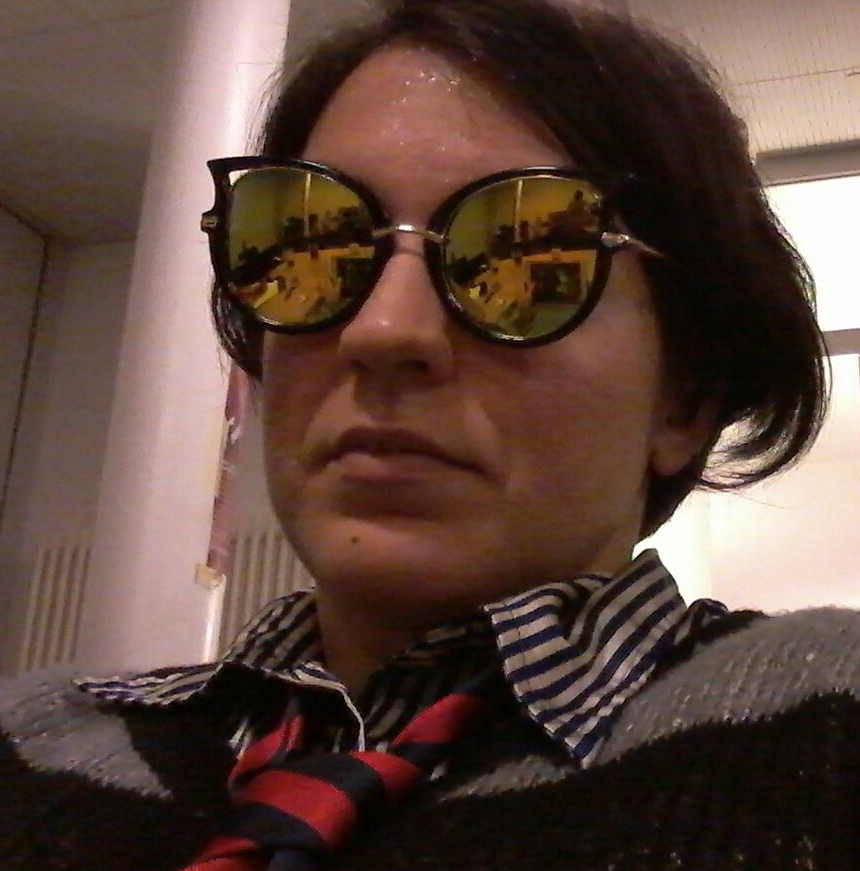
\includegraphics[height=2.60cm]{photo_2018}} &
        \begin{tabular}{l|p{5cm}}
    \raisebox{0pt}{\Smiley} & \textbf{Ariadni-Karolina Alexiou} \\ % Name
            \raisebox{-1pt}{\textifsymbol{18}}& 17 Bessemer Place, London SE \\ % Address
    \raisebox{-1pt}{\Letter} & carolinegr@gmail.com \\ % Email address
    \Keyboard & \href{http://www.github.com/carolinux}{http://www.github.com/carolinux} \\ % Github
        \end{tabular}  \\ % Name
\end{tabular}
}
}\\[10pt]







%----------------------------------------------------------------------------------------
%	COMPUTER SKILLS
%----------------------------------------------------------------------------------------

\section{Work Experience Contd.} 
{\raggedleft\textsc{November 2015 - February 2017}\par}
{\raggedright\large \textbf{Lead Data Engineer at Tracktics GmbH, Z\"urich}\\
}
\normalsize{Responsible for overseeing the extracting of insights from GPS and sensor data, collected from a tracker worn by football players in the field.}
\begin{itemize}
\item[$\bullet$] Built the production data pipeline. It automatically processed the raw data (various stages, eg:  MATLAB binary, Jupyter notebooks and python modules, chained together with celery)
\item[$\bullet$] Launched various additional tools (heatmap generator, football pitch locator) to production
\item[$\bullet$] Designed and oversaw the collection of test data to evaluate our algorithms
\item[$\bullet$] Built evaluation into the data pipeline (in a way that externals could use it, and internals could easily create new report templates for new metrics)
\item[$\bullet$] Built a library of common functionality together with the data scientists and mentored junior engineers
\end{itemize}

{\raggedleft\textsc{September 2013 - June 2015}\par}
{\raggedright\large \textbf{Software Engineer at Teralytics AG, Z\"urich}\\
}
\normalsize{Worked as a software engineer, extracting insights from mobile phone data and supporting my colleagues to do so.}
\begin{itemize}
\item[$\bullet$] Created data pipelines to go from raw data to automatically updating web dashboards in production 
\item[$\bullet$] Created interactive visualizations of geospatial data (using PostGIS, d3, QGIS) for our customers
\item[$\bullet$] Contributed to (and became co-maintainer) of an \href{http://github.com/anitagraser/TimeManager}{open source tool} to visualize geotemporal data
\item[$\bullet$] Built a library to unify access to diverse data sources
\end{itemize}
%\normalsize{\textbf{Geospatial Data} - Familiar with PostGIS, QGIS and have co-authored a \href{http://github.com/anitagraser/TimeManager}{plugin for interactive visualization of geotemporal data.}}\\

%Languages
%& \textsc{Python}, \textsc{Java}, \textsc{Scala} \\
%& \textsc{C/C++}, \textsc{VHDL}, \textsc{SQL} \\
%& \textsc{PHP}, \textsc{HTML}, \textsc{bash} \\
%& \textsc{JavaScript}, \textsc{\LaTeX} \\
%&\\
%Frameworks
%& Hadoop, Spark, pandas \\
%& Redis, MongoDB, PostgreSQL \\
%& JQuery, d3 \\
%& Boost, CGAL \\
%& Adobe Flash, FlashDevelop \\
%& MATLAB, R, QGIS \\
%& Open Office, Eclipse, IDEA, Vim\\


%\end{tabular}






%----------------------------------------------------------------------------------------
%	COMMUNICATION SKILLS
%----------------------------------------------------------------------------------------

%2010 (athens)	
%Volunteer in the 6th Hellenic Conference on Artificial Intelligence
%2008 – 09 (athens)	 Participation in Microsoft Imagine Cup
%2008 (samos)	 Panhellenic Conference on Informatics
%2008 (athens)	 3IA International Conference on Computer Graphics

\section{Selected Conferences and Articles} 

\begin{tabular}{rl}
\textsc{2017}
& Speaker at PyData Berlin conference:\\
& Patterns for Collaboration between Data Scientists\\
& and Software Engineers \\
& \href{https://www.youtube.com/watch?v=7oxC7cbRYyE}{video} | \href{https://www.codementor.io/blog/data-scientists-collab-5ah55wy1ro}{article} \\
\textsc{2016}
& Published reflections on the future of \href{http://www.datasciencecentral.com/profiles/blogs/interview-with-karolina-alexiou-building-data-pipelines}{Data Pipelines}\\
& and the future of \href{https://blog.propulsionacademy.com/why-python-for-data-science-is-the-future-b556de75c80c#.mdh3ztapq}{Python for Data Science}\\
\textsc{2015}
    & Tutorial (Python): \href{https://www.airpair.com/python/posts/using-python-and-qgis-for-geospatial-visualization}{Exploring a UFO sightings dataset}\\
\textsc{2015}
& Article: \href{https://www.airpair.com/python/posts/top-mistakes-python-big-data-analytics}{Common mistakes with Python and Big Data}\\
\textsc{2015}
& Workshop on visualizing geotemporal data\\
\textsc{2014}
& Presented published paper at VLDB 2014\\
\textsc{2014}
& Speaker at PyData Berlin conference \\
& on Mall Analytics (from prototype to product) \\ 
%\textsc{2014}
%& Speaker at \\
%& Swiss Postgres conference \\
%& \small Rapperswil, Switzerland \\
%\textsc{2014}
%& Speaker at \\
%& Swiss Big Data User Group Meetup \\
%& \small Z\"urich, Switzerland \\


%\textsc{2009}
%& Participated in Microsoft Imagine Cup \\
%&\small  Athens, Greece\\



\end{tabular}\\[10pt]

	
\end{minipage} % End right-hand side of the page

% teh second page!
\begin{minipage}[t]{0.5\textwidth} % Start the left-hand side of the page
\vspace{0pt} % Trick for alignment
	
%----------------------------------------------------------------------------------------
%	EDUCATION
%----------------------------------------------------------------------------------------

\section{Education} 

\begin{tabular}{rl} % Start a table with two columns, one for dates and one for qualifications



2011 -- 2013 & \textbf{Master of Science} \\ 
& \textsc{Computer Science} \\ 
& \textit{ETH Z\"urich}\\
    \small  & GPA: 5.5/6 (also received scholarship) \\
2007 -- 2011 & \textbf{Bachelor of Science}\\
& \textsc{Computer Science} \\
& \textit{University of Athens} \\
\small  & GPA: 9.3/10 -- Top graduate in fall 2011\\
	
\end{tabular}\\[9pt]


\section{Selected Freelance or Other Work} 


{\raggedright\large \textbf{Node Developer for SignedBlock, Athens}\\
}

\normalsize{Extended and dockerized a program for live collection of data from the cryptocurrency market.}
\\

{\raggedright\large \textbf{QGIS Plugin Developer for OpenGis.ch, Z\"urich}\\
}

\normalsize{Responsible for developing Python plugins for geospatial data management.}\\

{\raggedright\large \textbf{Python and Data Engineering Tutor, online}\\
}

\normalsize{Micro-consulting via \href{http://www.codementor.io/carolinux}{codementor.io} on several data science/engineering projects.}\\

{\raggedright\large \textbf{Mentor at Andela, online}\\
}

\normalsize{Mentored junior programmers in Python, testing and programming patterns to prepare them for working remotely.} 
\\

{\raggedright\large \textbf{Data Consultant for New Incentives, Z\"urich}\\
}

\normalsize{Created a data pipeline in Scala to sync data daily across mobile devices and Google spreadsheets.}\\

{\raggedright\large \textbf{Software Engineering Intern, Google Z\"urich}\\
}

\normalsize{Migrated a feature of Youtube Analytics to the new backend.}\\

%------------------------------------------------
% WORK EXPERIENCE 2
%------------------------------------------------

%{\raggedleft\textsc{February 2012 -- May 2012}\par}

%{\raggedright\large \textbf{Teaching Assistant for the Data Modeling and Databases course at ETH, Zurich}\\}

%\normalsize{Taught basic and intermediate concepts of databases (eg. UML, Relational Models, Normal Forms, Transactions, SQL operators), created exercises for students and graded their final SQL and Java projects.}\\

%------------------------------------------------
% WORK EXPERIENCE 3
%------------------------------------------------

%{\raggedleft\textsc{March 2011 -- June 2011}\par}

%{\raggedright\large \textbf{Game programmer at 4pi Publications, Athens}\\}

%\normalsize{Created flash games for an educational magazine in ActionScript 3.0, working closely with sound and graphic artists.}\\


%----------------------------------------------------------------------------------------
	

\end{minipage} % End the left-hand side of the page
\hfill
\begin{minipage}[t]{0.44\textwidth} % Start the right-hand side of the page
\vspace{0pt} % Trick for alignment


\section{Languages} 
\normalsize{English, German and Spanish in full professional capacity. Greek as mother tongue, some French.}\\

\section{Personal Interests} 
    \normalsize{Painting (have some professional training), Social Science, Traveling. I have combined my thinking/practice as a programmer with those of being an artist to create a \href{https://medium.com/@_sandtweets/learn-drawing-and-programming-at-the-same-time-at-mozfest-2017-6a9f8627b72}{Drawing for Techies Workshop}, which I have run multiple times in Switzerland, Germany and the UK.}\\
%----------------------------------------------------------------------------------------
	
\end{minipage} % End right-hand side of the page

\end{document}  
